\section{Prototipo 2: Generador de Registros Artificiales (GRA)}
En la sección actual se encuentra el análisis, diseño y pruebas del prototipo del módulo Generador de Registros Artificiales; este se encarga de insertar registros en múltiples tablas de la base de datos del sistema.\\

\subsection{Análisis}


%%%%%%%%%%%%%%%%%%%%%%%%%%%%%%%%%%%%%%%%%%%%%%%%%%%%%%%%%%%%%%%%%%%
\title{\textbf{Diagrama de casos de uso}\\}
En la figura \ref{image:casosusoGRA} se muestra el diagrama de casos de uso del módulo Generador de Registros Artificiales.

\FloatBarrier
\begin{figure}[htbp!]
		\centering
			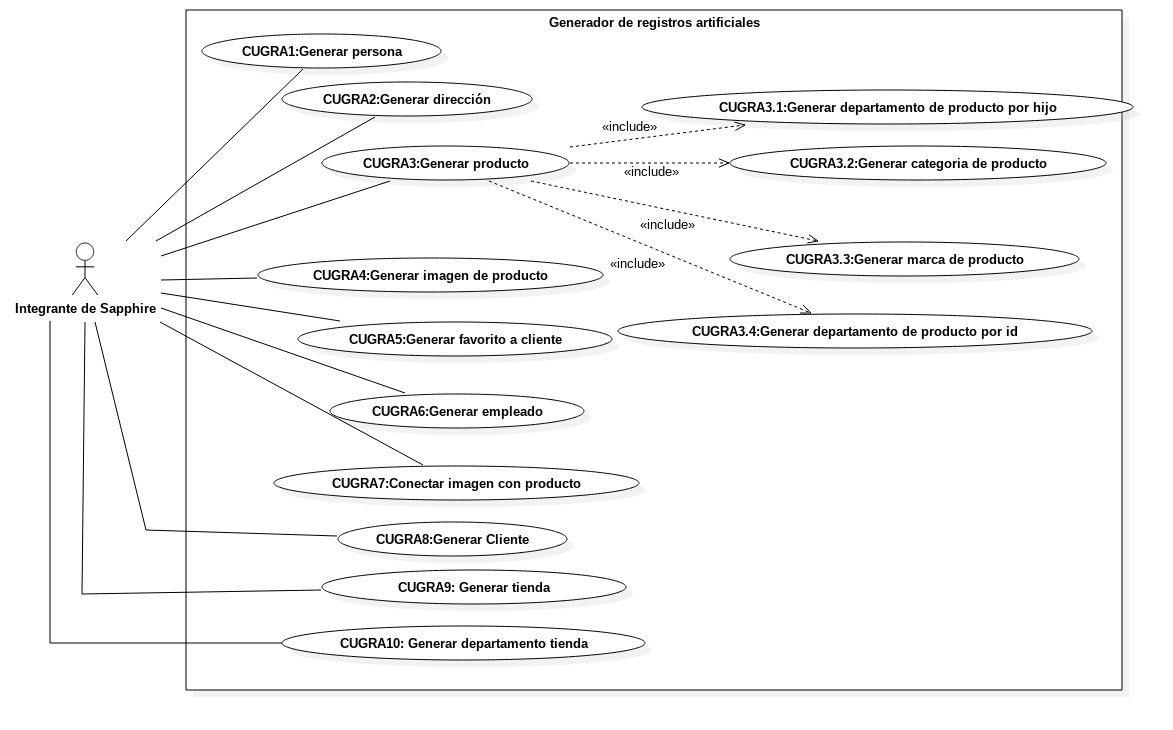
\includegraphics[width=.9 \textwidth]{imagenes/CU/generadorRegistros}
		\caption{Diagrama de casos de uso módulo Generador de Registros Artificiales.}
		\label{image:casosusoGRA}
\end{figure}
\FloatBarrier


\title{\textbf{Diagrama de clases}\\}
La descripción de los elementos en el diagrama de clases (figura \ref{image:diagramaclasesGRA}) es la siguiente: 

\begin{itemize}
\item \textbf{Generator}: Clase encargada de la interacción con el usuario, muestra el menú y lee la opción ingresada por el usuario.
\item \textbf{FakerGenerator}: Clase engargada de tener la lógica para generar los registros artificiales.
\item \textbf{MysqlConnection}: Clase encargada de manejar la comunicación entre el módulo GRA y el gestor de base de datos MySQL.
\item \textbf{PsqlConnection}: Clase encargada de manejar la comunicación entre el módulo GRA y el gestor de base de datos PostgreSQL.
\end{itemize}

\FloatBarrier
\begin{figure}[htbp!]
		\centering
			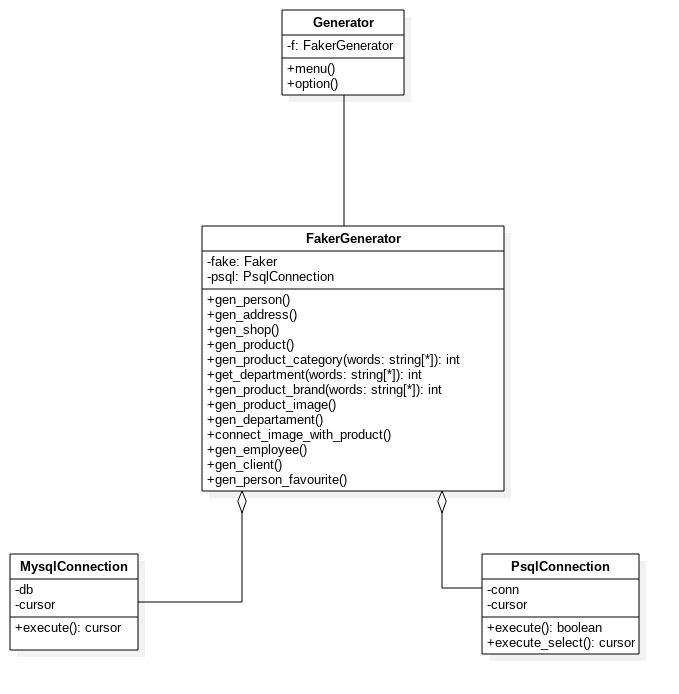
\includegraphics[width=.7 \textwidth]{imagenes/ClasesRuben/generador}
		\caption{Diagrama de clases de módulo Generador de Registros Artificiales.}
		\label{image:diagramaclasesGRA}
\end{figure}
\FloatBarrier

\subsection{Diseño}

\title{\textbf{Diagramas de secuencia\\}}
Durante este apartado se realizará una pequeña explicación de cada método dentro de la clase FakerGenerator, además, dentro del mismo se muestran los diagramas de secuencia de dichos métodos separados dentro de sus respectivos apartados. \\






\title{\textbf{Generar persona\\}}
Método encargado de cubrir el requerimiento funcional \textbf{RFGRA2} que permite realizar el registro de personas ficticias en el repositorio de datos. En la figura \ref{image:DSgenerarPersona} se muestra su diagrama de secuencia. 
\FloatBarrier
\begin{figure}[htbp!]
		\centering
			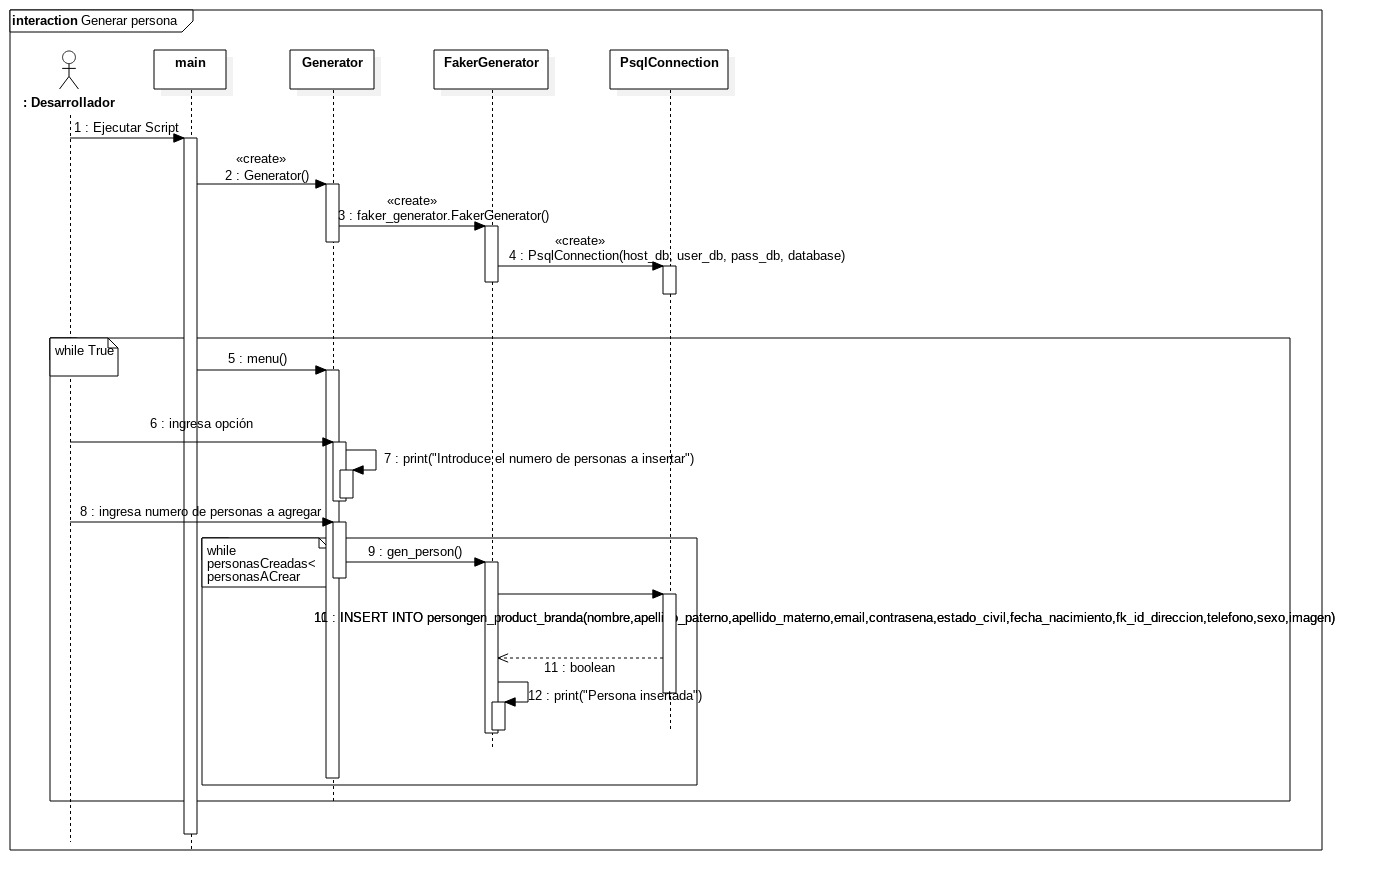
\includegraphics[width=1.1 \textwidth]{imagenes/DSRuben/gen_person_generator}
		\caption{Diagrama de secuencia para generar persona.}
		\label{image:DSgenerarPersona}
\end{figure}
\FloatBarrier





\title{\textbf{Generar dirección\\}}
En el diagrama de secuencia que se muestra en la figura \ref{image:DSgenerarDireccion} se muestra la interación del método encargado de generar direcciones ficticias que satisfacen el requerimiento funcional \textbf{RFGRA3}.
\FloatBarrier
\begin{figure}[htbp!]
		\centering
			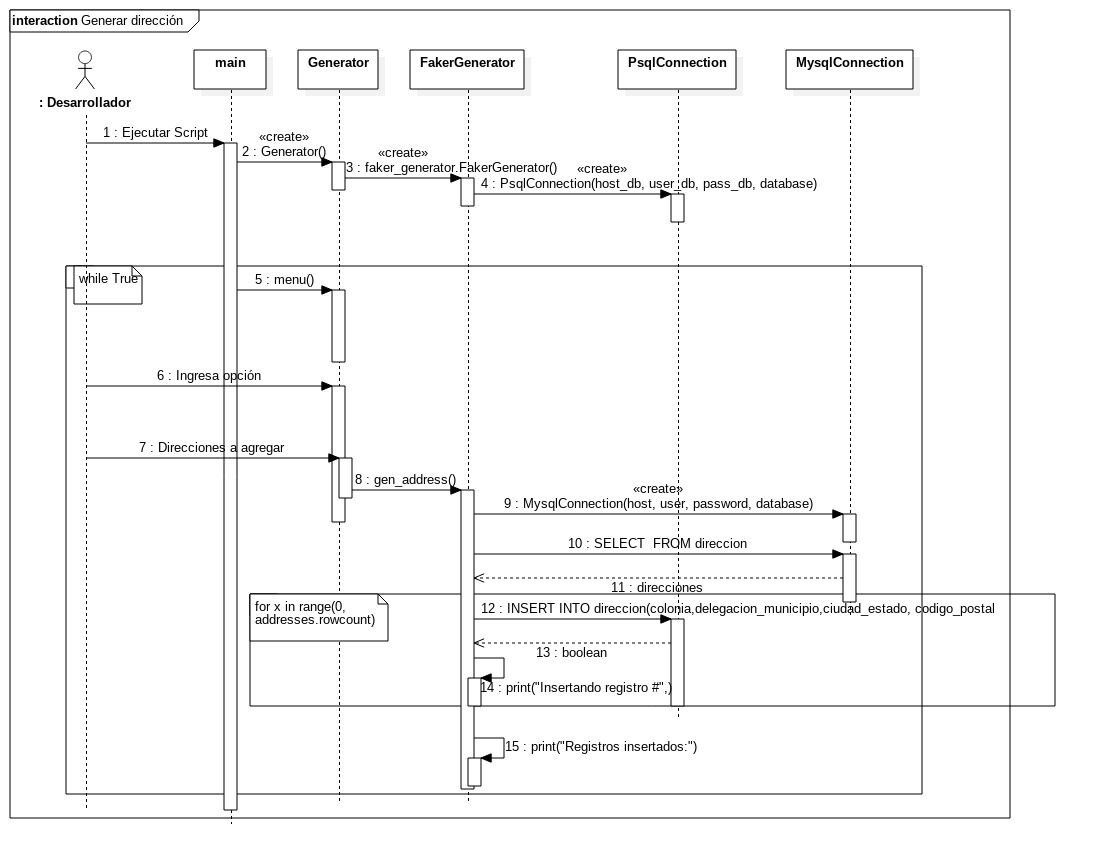
\includegraphics[width=1.1 \textwidth]{imagenes/DSRuben/gen_address_generator}
		\caption{Diagrama de secuencia para generar dirección.}
		\label{image:DSgenerarDireccion}
\end{figure}
\FloatBarrier







\title{\textbf{Generar tienda}}
\FloatBarrier
Método encargado de cubrir el requerimiento funcional \textbf{RFGRA4} que permite generar establecimientos comerciales ficticios y posteriormente registrarlos en el repositorio de datos. La figura \ref{image:DSGenerarTienda} se muestra su diagrama de secuencia. 
\begin{figure}[htbp!]
		\centering
			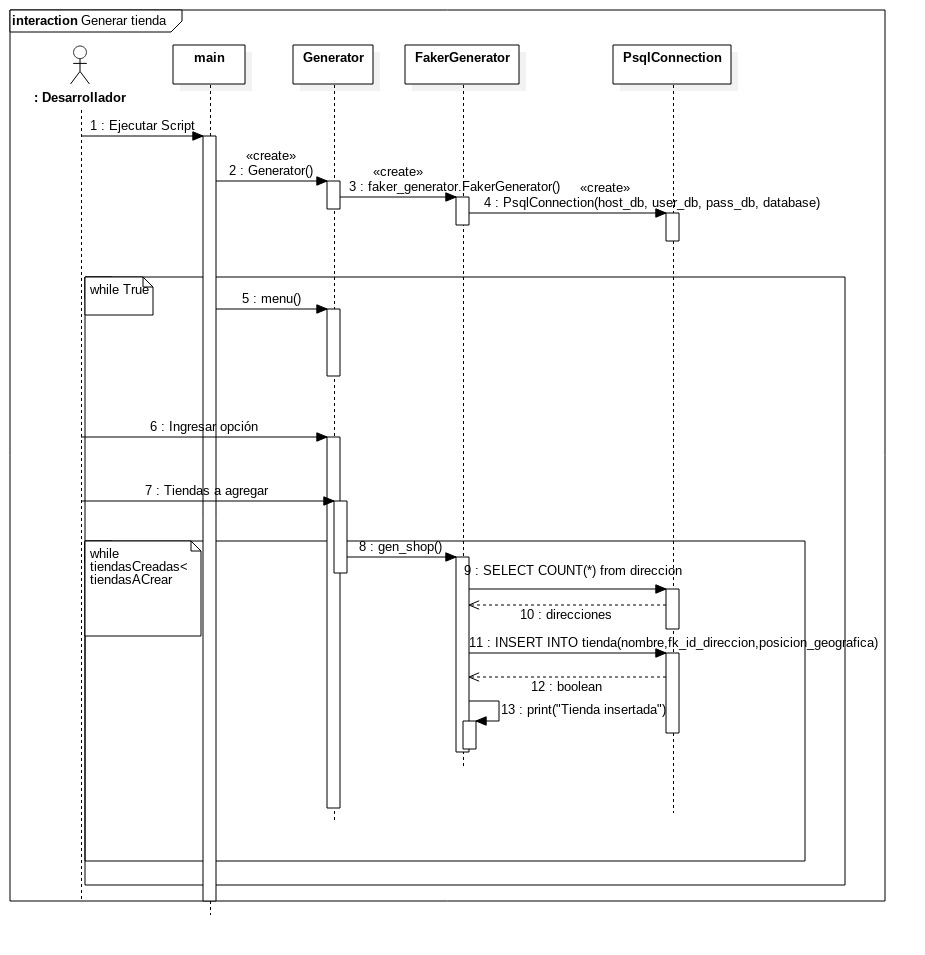
\includegraphics[width=1 \textwidth]{imagenes/DSRuben/gen_shop_generator}
		\caption{Diagrama de secuencia para generar tienda.}
		\label{image:DSGenerarTienda}
\end{figure}
\FloatBarrier






\title{\textbf{Generar departamento\\}}
En el diagrama de secuencia que se muestra en la figura \ref{image:DSGenerarDepartamento} se muestra la interación del método encargado de generar direcciones ficticias que satisfacen el requerimiento funcional \textbf{RFGRA5}.
\FloatBarrier
\begin{figure}[htbp!]
		\centering
			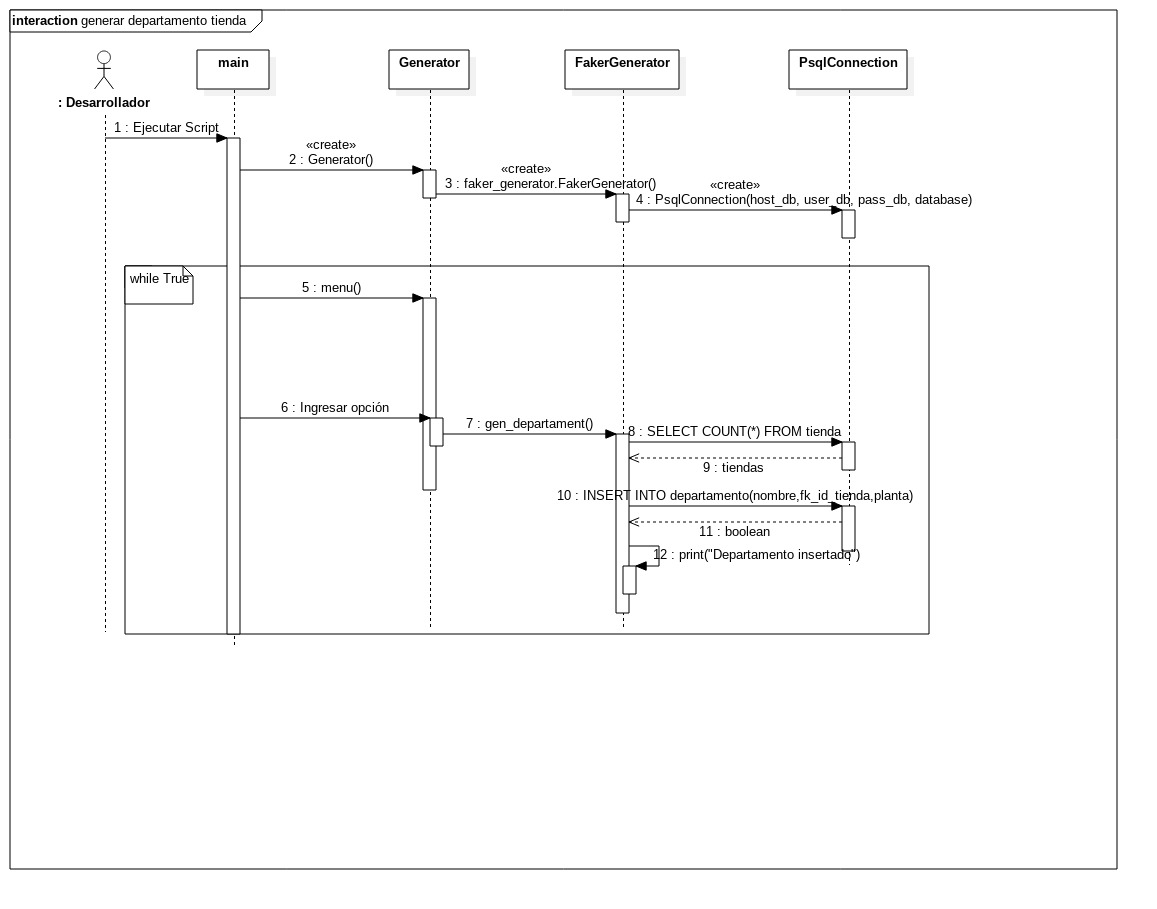
\includegraphics[width=1 \textwidth]{imagenes/DSRuben/gen_department_generator}
		\caption{Diagrama de secuencia para generar departamento.}
		\label{image:DSGenerarDepartamento}
\end{figure}
\FloatBarrier





\title{\textbf{Generar producto\\}}
En el siguiente diagrama (Figura \ref{image:DSGenerarProducto}) se muestra la interacción del método creado con el objetivo de insertar productos en el repositorio de datos que satisface el requerimiento funcional \textbf{RFGRA6}. Cabe mencionar que este método hace uso de los  casos de uso \textbf{CUGRA3.1,CUGRA3.2,CUGRA3.3,CUGRA3.4} y por lo tanto se encuentran inmersos en el diagrama de secuencia.  
\FloatBarrier
\begin{figure}[htbp!]
		\centering
			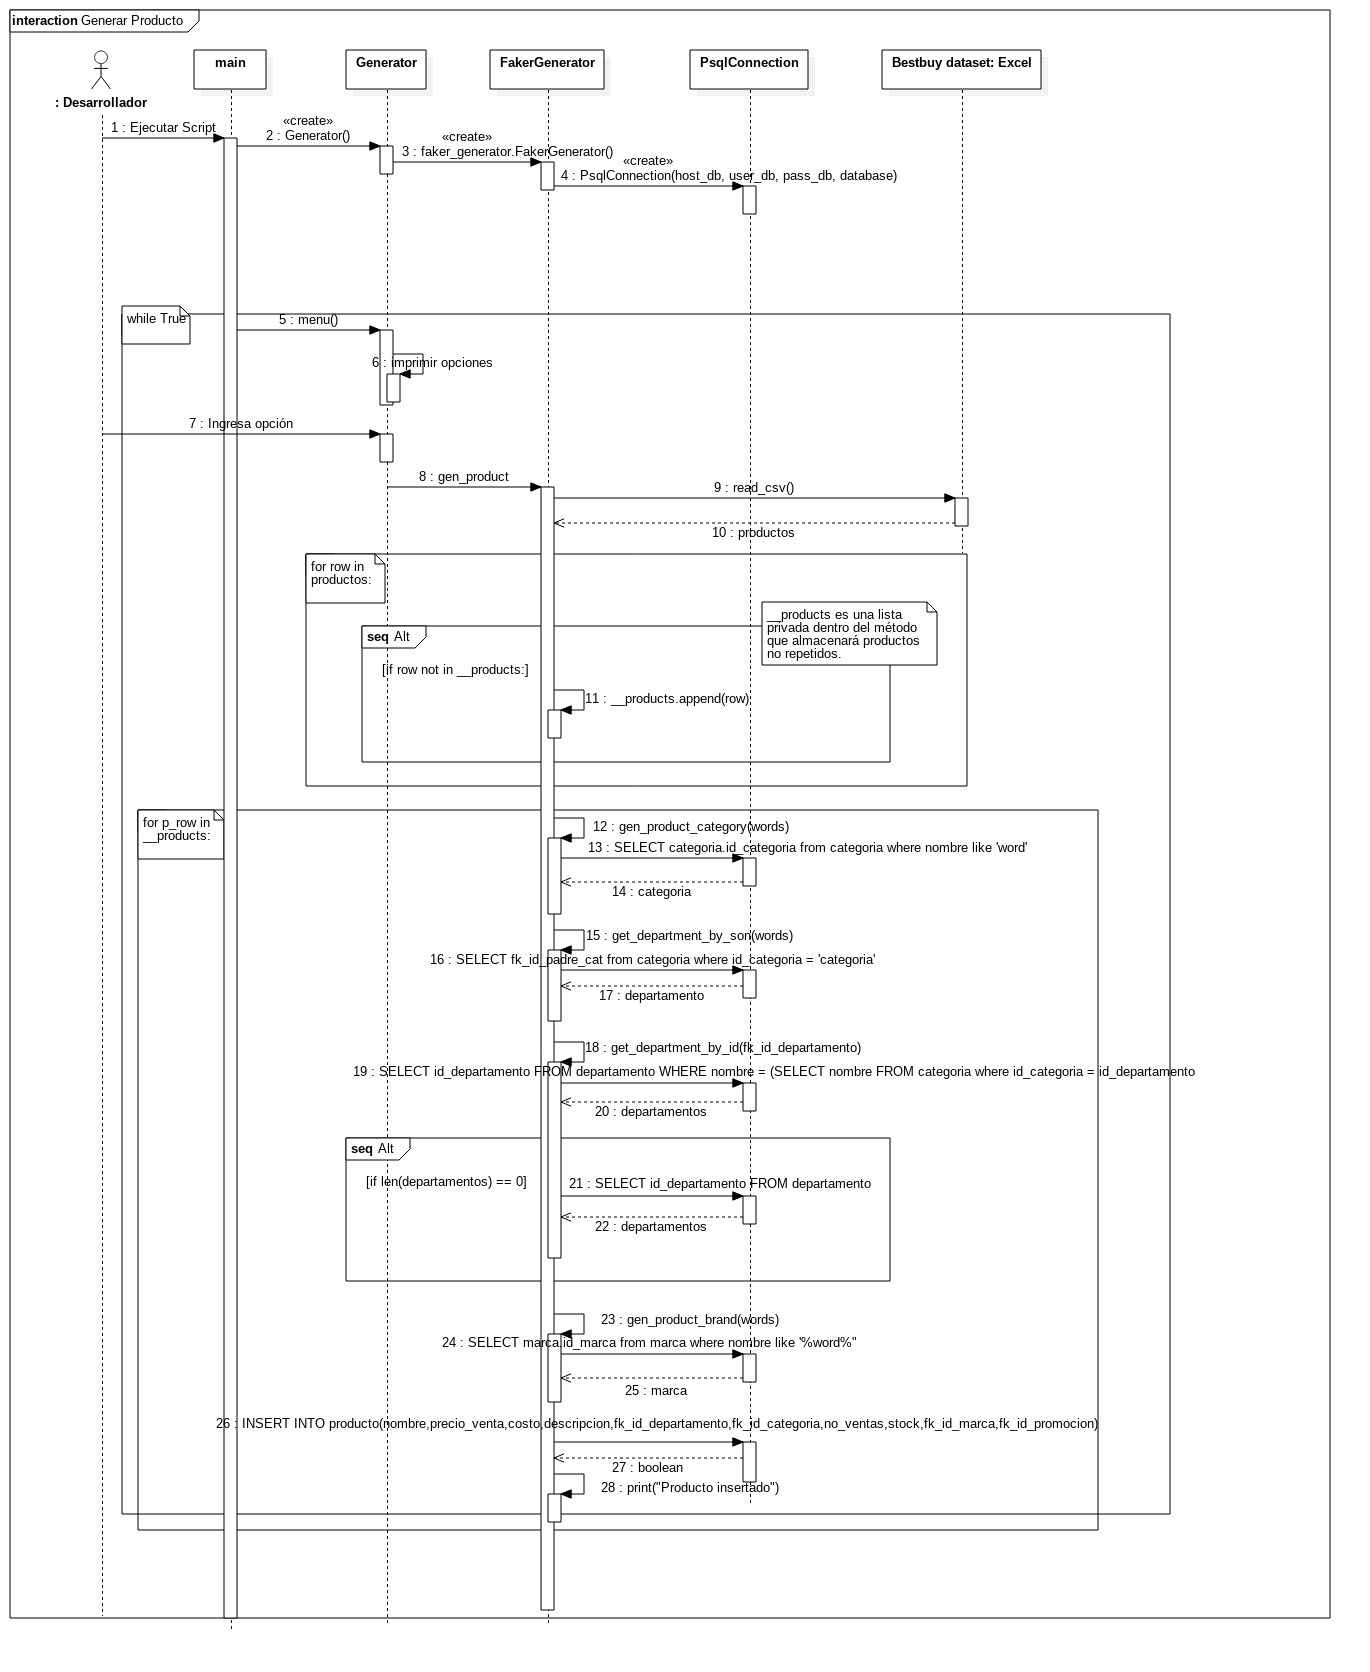
\includegraphics[width=1 \textwidth]{imagenes/DSRuben/gen_product_generator}
		\caption{Diagrama de secuencia para generar producto.}
		\label{image:DSGenerarProducto}
\end{figure}
\FloatBarrier




\title{\textbf{Generar imágenes pertenecientes a productos\\}}
En el diagrama de secuencia que se muestra en la figura \ref{image:DSGenerarImagenesAProductos} se muestra la interación del método encargado de insertar imágenes en el repositorio de datos que satisfacen el requerimiento funcional \textbf{RFGRA7}.
\FloatBarrier
\begin{figure}[htbp!]
		\centering
			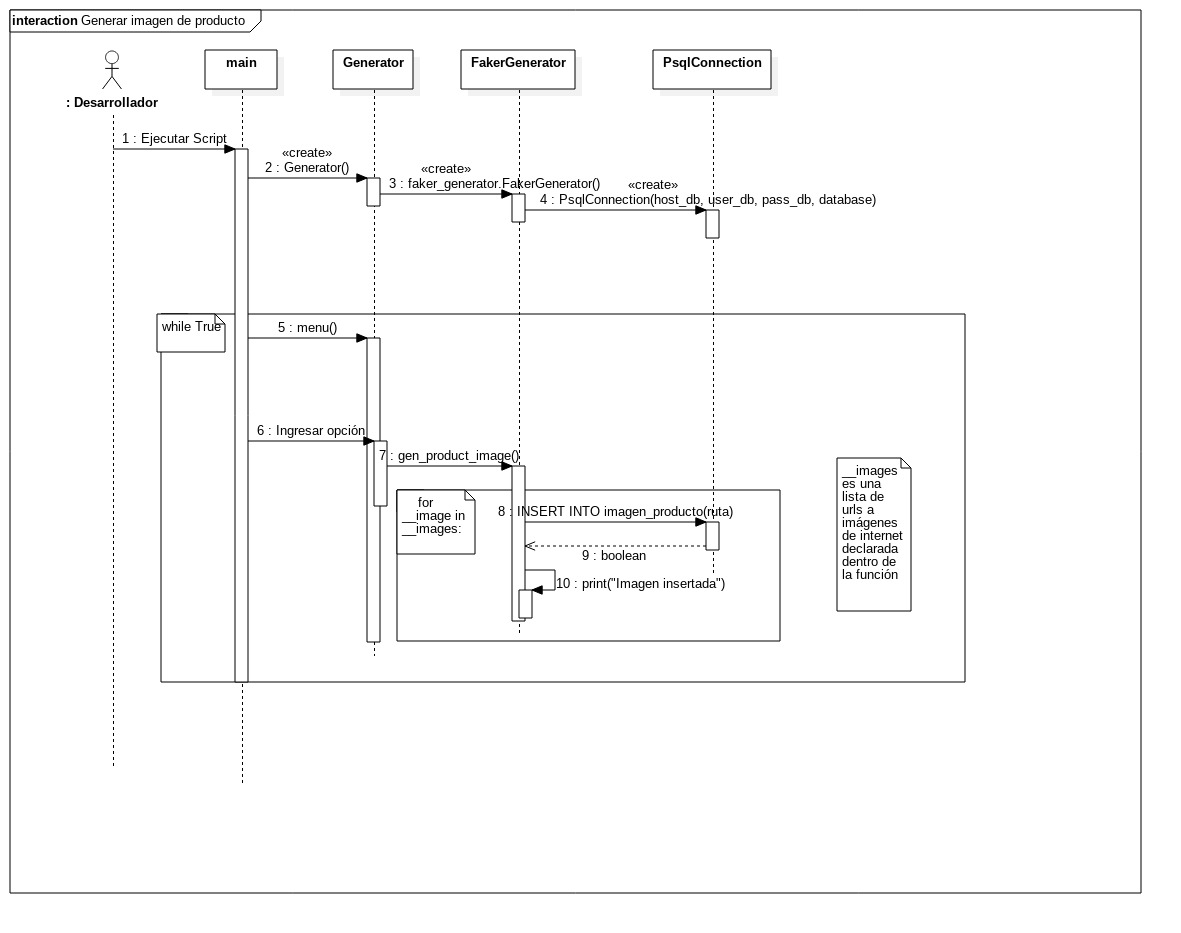
\includegraphics[width=1.1 \textwidth]{imagenes/DSRuben/gen_product_image_generator}
		\caption{Diagrama de secuencia para generar imágenes pertenecientes a productos.}
		\label{image:DSGenerarImagenesAProductos}
\end{figure}
\FloatBarrier





\title{\textbf{Asignar imágenes a productos \\}}
Este método se encarga de asignar imágenes a productos de manera aleatoria. El diagrama de secuencia se puede apreciar en la figura \ref{image:DSAsignarImagenesAProductos}. Cabe mencionar que este método satisface el requerimiento funcional \textbf{RFGRA8}.
\FloatBarrier
\begin{figure}[htbp!]
		\centering
			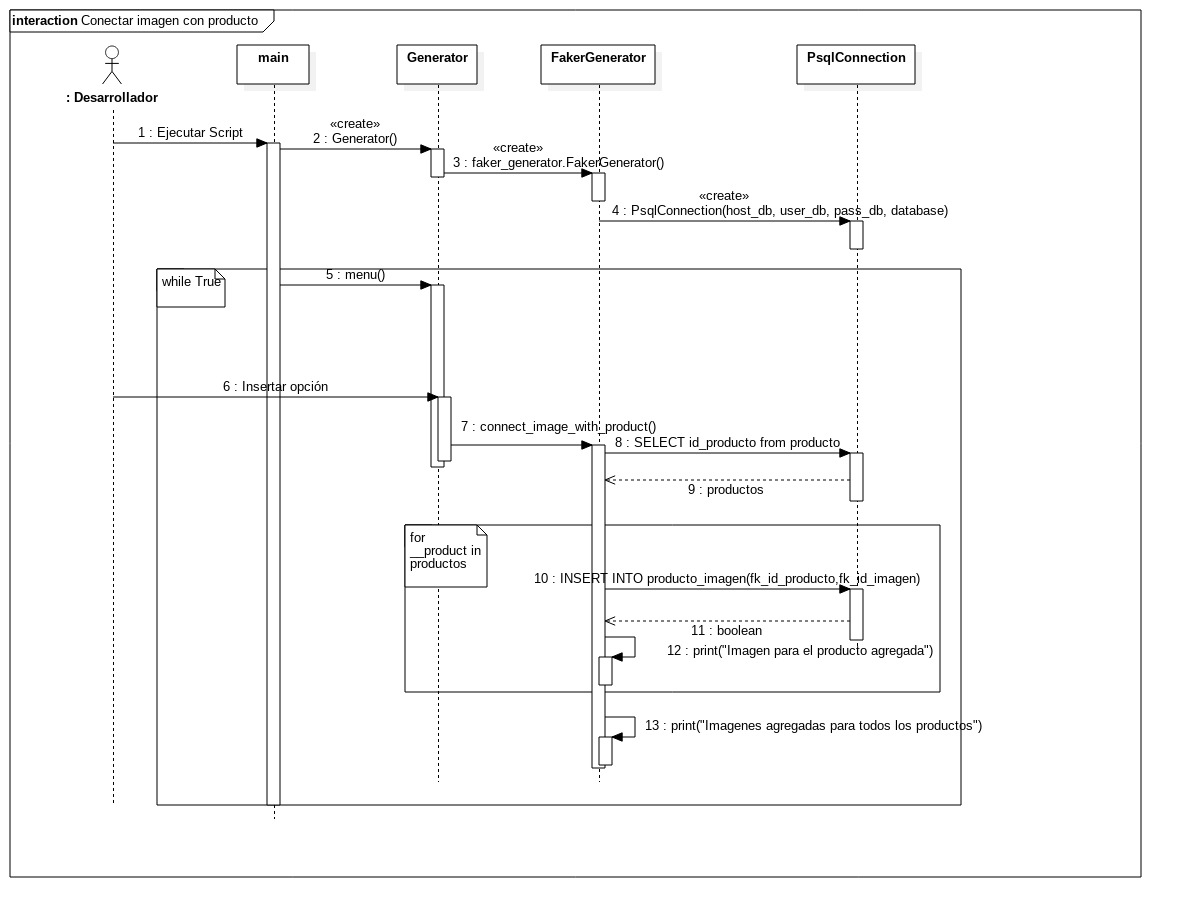
\includegraphics[width=1.1 \textwidth]{imagenes/DSRuben/connect_image_with_product_generator}
		\caption{Diagrama de secuencia para asignar imágenes a productos.}
		\label{image:DSAsignarImagenesAProductos}
\end{figure}
\FloatBarrier




\title{\textbf{Generar empleados \\}}
Método creado con el objetivo de crear empleados con las personas ficticias que han sido registradas anteriormente por el método para generar personas; este método satisface el requerimiento funcional \textbf{RFGRA9} y su respectivo diagrama de secuencia se encuentra en la figura \ref{image:DSGenerarEmpleados}.
\FloatBarrier
\begin{figure}[htbp!]
		\centering
			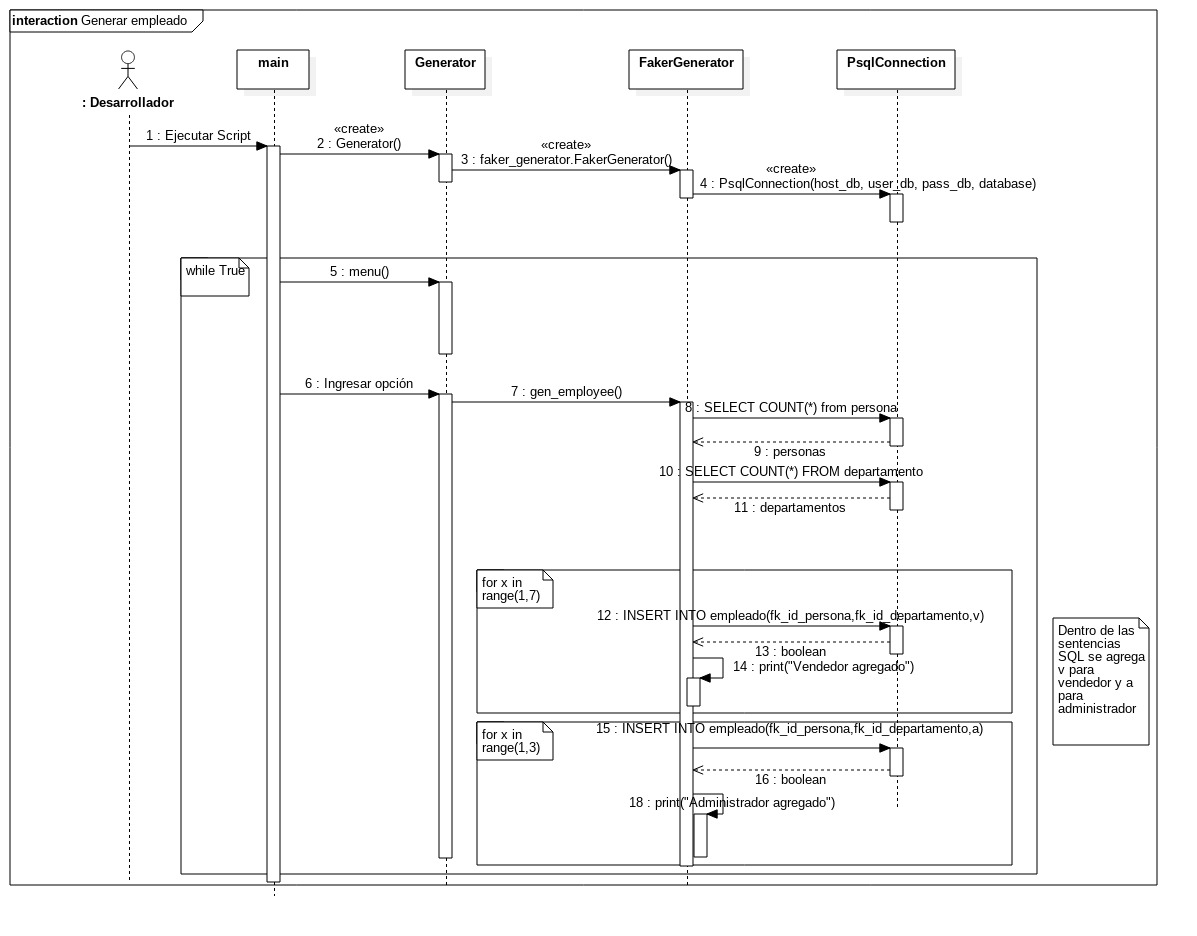
\includegraphics[width=1.1 \textwidth]{imagenes/DSRuben/gen_employee_generator}
		\caption{Diagrama de secuencia para generar empleados.}
		\label{image:DSGenerarEmpleados}
\end{figure}
\FloatBarrier





\title{\textbf{Generar clientes\\}}
En el diagrama de secuencia que se muestra en la figura \ref{image:DSGenerarClientes} muestra la interación del método encargado de generar clientes ficticios  que satisfacen el requerimiento funcional \textbf{RFGRA10}.

\FloatBarrier
\begin{figure}[htbp!]
		\centering
			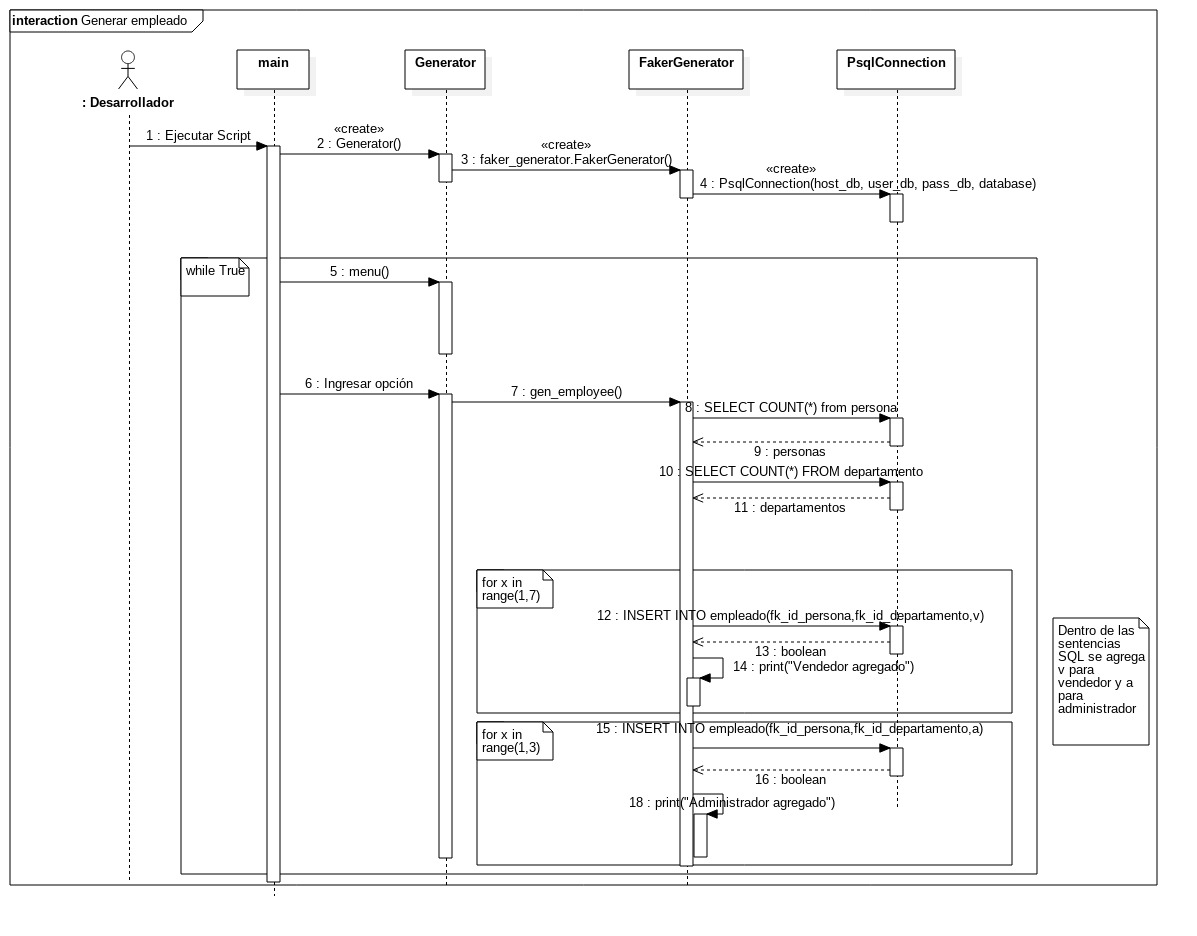
\includegraphics[width=1 \textwidth]{imagenes/DSRuben/gen_employee_generator}
		\caption{Diagrama de secuencia para generar clientes.}
		\label{image:DSGenerarClientes}
\end{figure}
\FloatBarrier




\title{\textbf{Asignar productos favoritos a clientes}}
Este método se encarga de asignar productos favoritos a clientes de manera que crea un patrón dentro de los datos. El diagrama de secuencia se puede apreciar en la figura \ref{image:DSAsignarFavoritosAClientes}. Cabe mencionar que este método satisface el requerimiento funcional \textbf{RFGRA11}.

\FloatBarrier
\begin{figure}[htbp!]
		\centering
			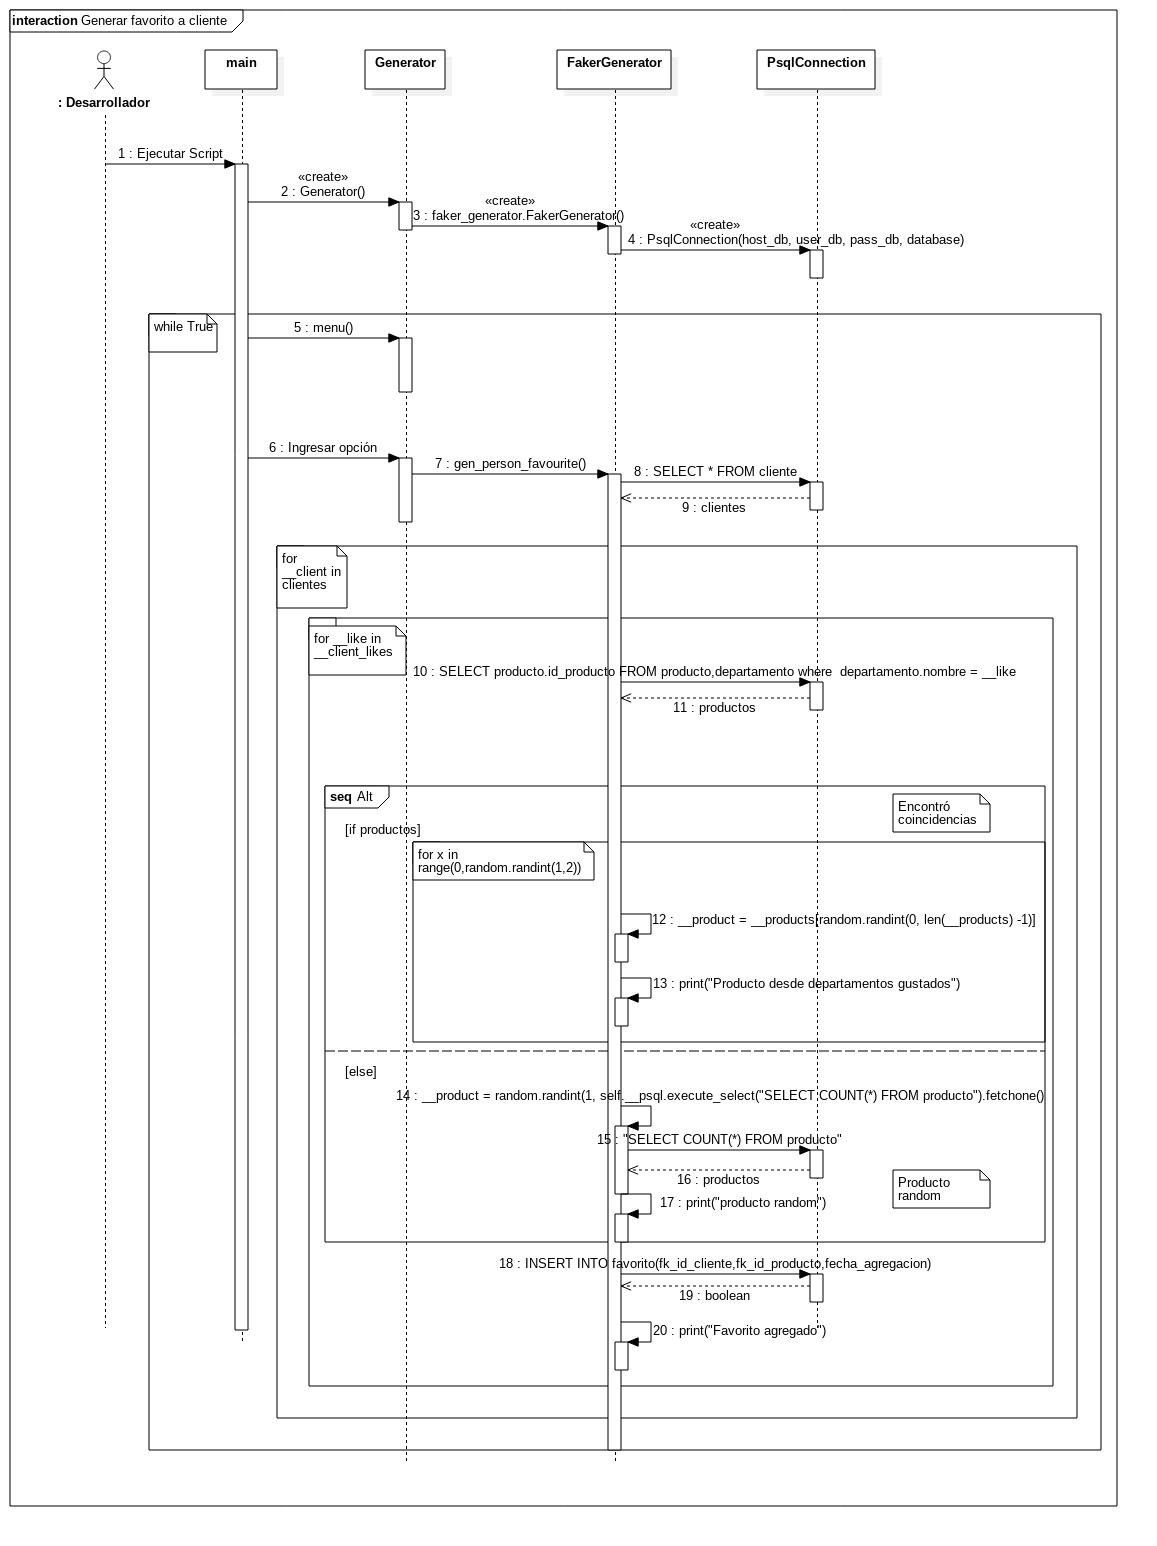
\includegraphics[width=1 \textwidth]{imagenes/DSRuben/gen_person_favourite_generator}
		\caption{Diagrama de secuencia para asignar productos favoritos a cliente}
		\label{image:DSAsignarFavoritosAClientes}
\end{figure}
\FloatBarrier

La Figura \ref{RA:1} muestra el menú del Generador de Registros Artificiales.

\FloatBarrier
\begin{figure}[htbp!]
		\centering
			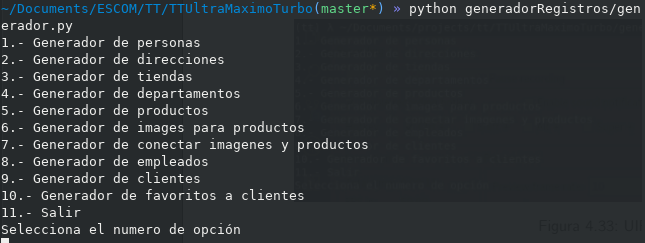
\includegraphics[width=.9 \textwidth]{imagenes/registrosArt/Menu}
		\caption{UIRA: Menú}
		\label{RA:1}
\end{figure}
\FloatBarrier




